\documentclass[11pt]{article}
\usepackage{fullpage}
\usepackage{graphicx}

\title{CS63 Spring 2024\\Predicting Emotions with GRUs}
\author{Alex Huynh, Branley Mmasi}
\date{May 6th, 2024}

\begin{document}

\maketitle

\section{Abstract}

Sentiment analysis—which is the ability to automatically detect and classify underlying sentiment expressed in text data—has become increasingly important across various domains. While traditional approaches such as rule-based methods and machine learning techniques can achieve high precision in certain contexts, they often fail to capture the nuances and complexities of natural language. In this paper, we propose a Gated Recurrent Unit (GRU)-based deep learning approach for sentiment analysis on a dataset of tweets. Our approach leverages the strengths of GRUs, which employ gating mechanisms to effectively model long-term dependencies in sequential data. The methodology involves tokenizing the text data, embedding the tokens into dense vector representations, and processing the embedded sequences using a GRU layer. The output of the GRU layer is then passed to a dense layer with a softmax activation function for sentiment classification. We evaluate the performance of our model using various metrics, including accuracy, confusion matrix, and word embeddings. Our proposed GRU model achieved an impressive accuracy of 93\% on the test set, demonstrating the suitability of our approach and outperforming a simple RNN or traditional methods. 

\section{Introduction}

The proliferation of user-generated content on social media platforms, online forums, and review websites has given rise to a vast amount of textual data containing valuable insights into people’s opinions, sentiments, and emotions. Extracting and analyzing these subjective expressions can provide businesses, organizations, and public sentiment on various topics of interest. Sentiment analysis, or option mining, seeks to computationally identify and classify the underlying sentiment polarity expressed in textual data with numerous applications, ranging from monitoring brand reputation and customer satisfaction to tracking public opinion on various topics.

As aforementioned, traditional approaches have relied on rule-based methods or machine learning techniques like Naive Bayes, Support Vector Machines (SVMs), and logistic regression. These methods treat text as a flat sequence of words and fail to model contextual and sequential information effectively—particularly in the presence of sarcasm, irony, or domain-specific expressions. In recent years, deep learning techniques, particularly Recurrent Neural Networks (RNNs) and their variants like Gated Recurrent Units (GRUs), have emerged as powerful tools for sentiment analysis. RNNs are well suited for processing sequential data, and GRUs employ gating mechanisms that enable them to capture long-term dependencies more efficiently. GRUs, by introducing gating mechanisms that control the flow of information through the network, allow gradients to propagate better over long sequences mitigating the vanishing gradient problem more effectively than RNNs. They also have a simpler architechture with fewer parameters compared to Long Short-Term Memory (LSTM) units, another popular RNN variant, making them computationally more effect and potentially easier to train. Given that GRUs have been shown to achieve comparable or even better performance than traditional RNNs and LSTMs on various natural language tasks, they became an obvious choice of study. In this paper, we propose a GRU-based deep learning approach for sentiment analysis on a dataset of tweets, leveraging techniques such as tokenization and word embeddings to overcome the limitations of traditional methods and more accurately capture the nuances of natural language.

\section{Methods}

The proposed GRU-based model was first implemented on Geeks for Geeks but on a binary classification problem and on a much smaller dataset. We implemented our model using TensorFlow and Keras libraries for Python, and adjusted it for categorical classification. The preprocessed dataset consisted of 70,000 tweets from Kaggle's Emotions dataset, with each tweet represented as a tuple containing the tweet text and its corresponding sentiment label (one of six emotions: sadness, joy, love, anger, fear, or surprise). The first step was tokenization, which involved converting the raw text into sequences of integer-encoded tokens. We utilized the Tokenizer class from the Keras preprocessing module, which constructs a vocabulary of the 5,000 most frequent words in the corpus. Each word in the vocabulary was assigned a unique integer index, while out-of-vocabulary words were represented by a special token. The tokenized text sequences were then padded or truncated to a fixed length which we set to 100. This ensured that all input sequences had a consistent length required for efficient batch processing during training. To capture semantic and contextual information about words, we employed an embedding layer that maps the integer-encoded tokens into dense vector representations. The embedding layer was initialized with random weights and learned these vector representations during the training process, such that semantically similar words were mapped to similar vector representations in the embedding space.

The sequence of embedded word vectors was then fed into a GRU layer, which processed the input sequence recurrently, capturing the long-term dependencies and contextual information within the text data. The GRU layer contained 128 units and used the hyperbolic tangent (tanh) activation function. The output of the GRU layer, which encapsulates the learned representations of the entire input sequence, was passed to a dense layer with a softmax activation function. This output layer produced a vector of six values, representing the probabilities of the input text belonging to each of the sentiment classes (sadness, joy, love, anger, fear, or surprise). The model was compiled using the categorical cross-entropy loss function and the Adam optimization algorithm. We split the dataset into training and test sets, with the first 60,000 examples used for training and 10,000 examples used for testing. We used a batch size of 256 and trained the model for 5 epochs, monitoring the validation loss and accuracy on the test set.

To evaluate the performance of our model, we utilized various metrics. We compared our model to one that uses a basic recurrent unit to observe the difference in performance between the two models. We utilized learning curves to check for evidence of overfitting. We compared embedding weights of similar words to observe what our model is learning. Lastly, we utilized a confusion matrix to identify areas of weakness in the model.

\section{Results \& Discussion}

\begin{figure}
    \begin{center}
    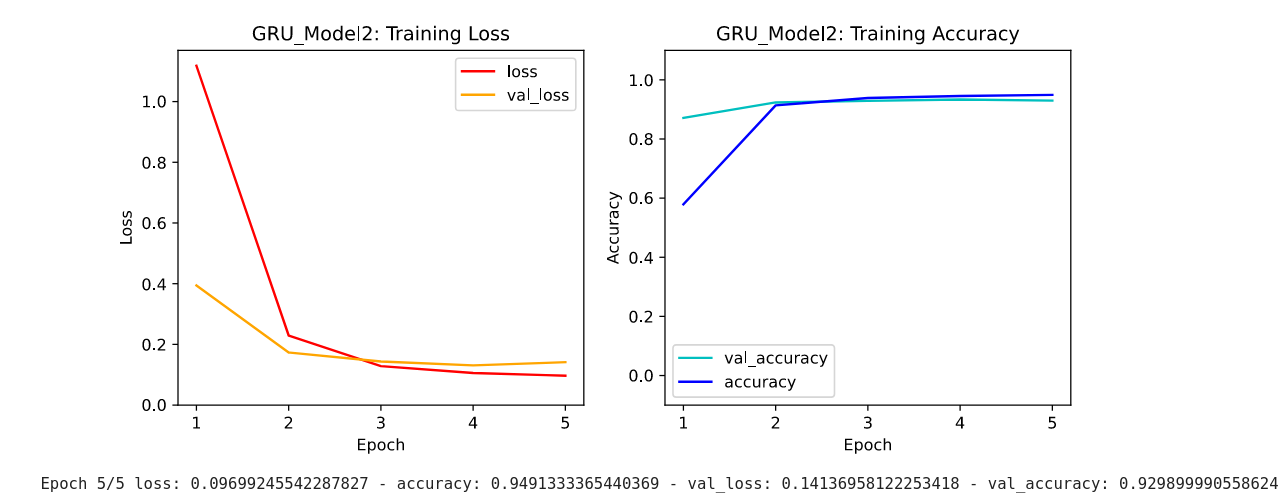
\includegraphics[width=8cm]{Model_2.png}
    \caption{Learning Curves for Model 2}
    \label{fig:height}
    \end{center}
\end{figure}

\begin{figure}
    \begin{center}
    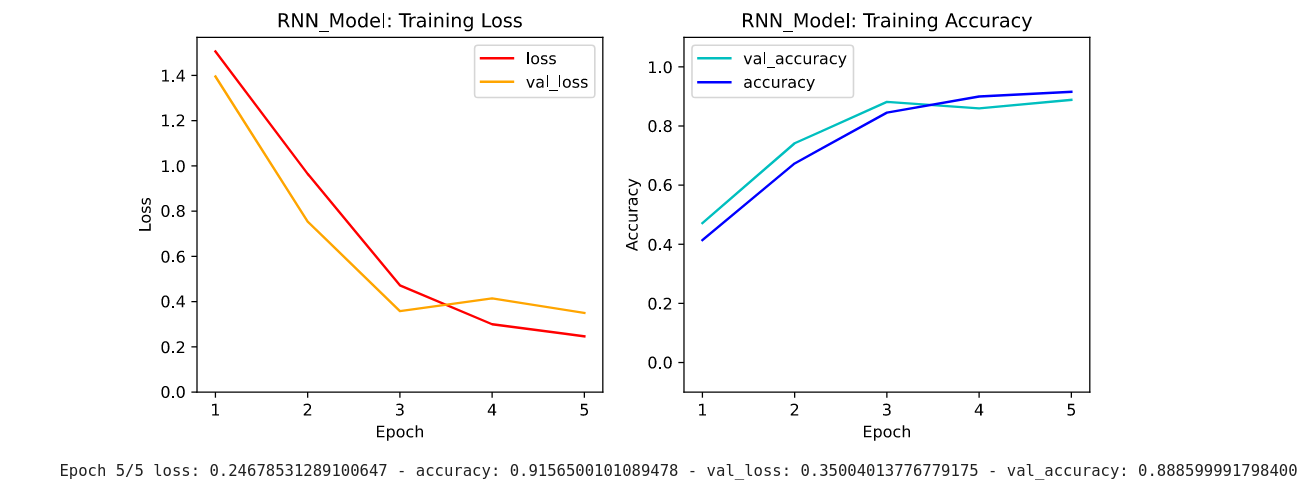
\includegraphics[width=8cm]{Model_3.png}
    \caption{Learning Curves for Model 3}
    \label{fig:height}
    \end{center}
\end{figure}

\begin{figure}
    \begin{center}
    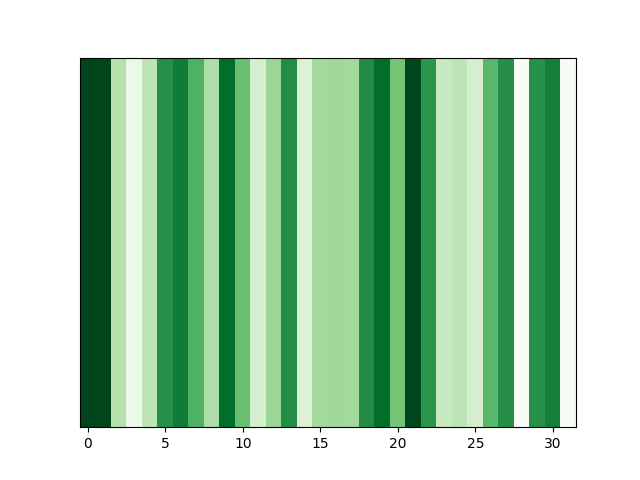
\includegraphics[width=8cm]{sad.png}
    \caption{Embedding of "Sad"}
    \label{fig:height}
    \end{center}
\end{figure}

\begin{figure}
    \begin{center}
    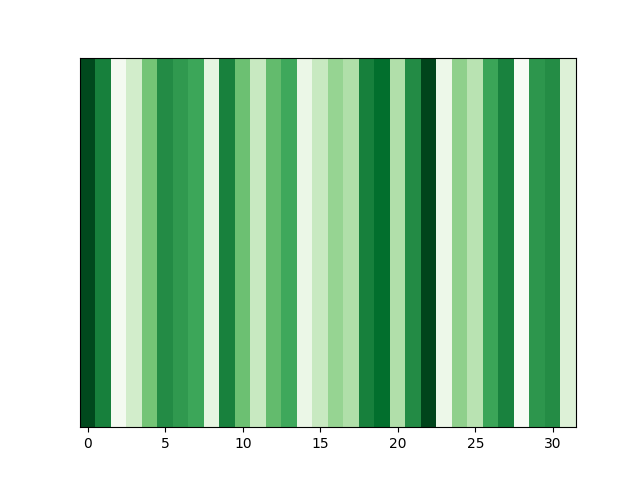
\includegraphics[width=8cm]{depressed.png}
    \caption{Embedding of "Depressed"}
    \label{fig:height}
    \end{center}
\end{figure}

\begin{figure}
    \begin{center}
    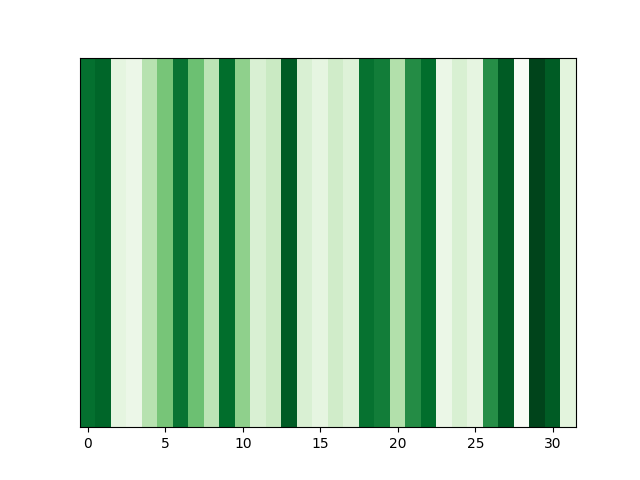
\includegraphics[width=8cm]{unhappy.png}
    \caption{Embedding of "Unhappy"}
    \label{fig:height}
    \end{center}
\end{figure}

\begin{figure}
    \begin{center}
    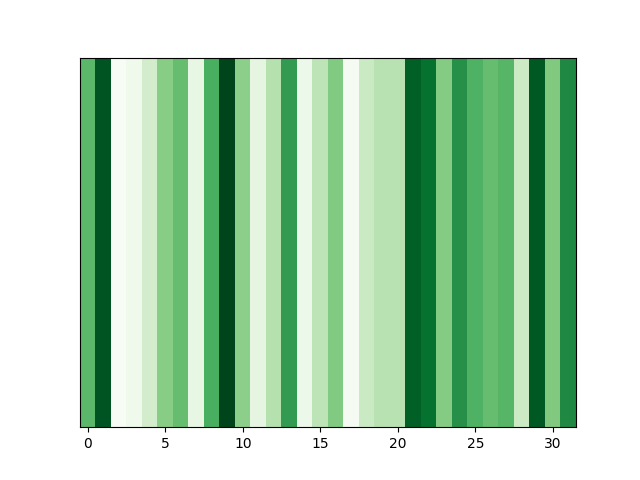
\includegraphics[width=8cm]{sadness.png}
    \caption{Embedding of "Sadness"}
    \label{fig:height}
    \end{center}
\end{figure}

\begin{figure}
    \begin{center}
    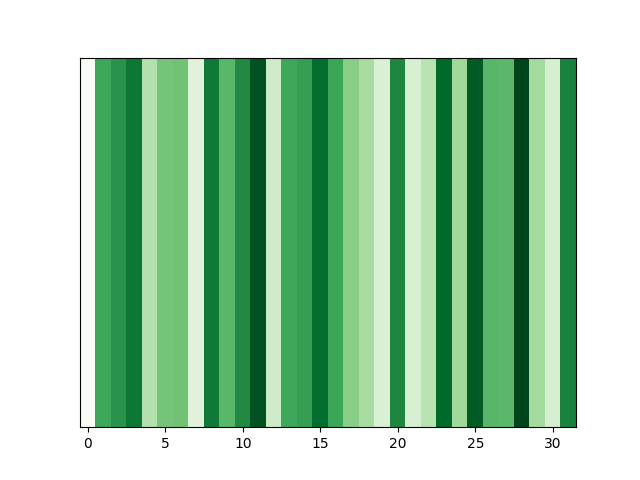
\includegraphics[width=8cm]{happy.png}
    \caption{Embedding of "Happy"}
    \label{fig:height}
    \end{center}
\end{figure}

\begin{figure}
    \begin{center}
    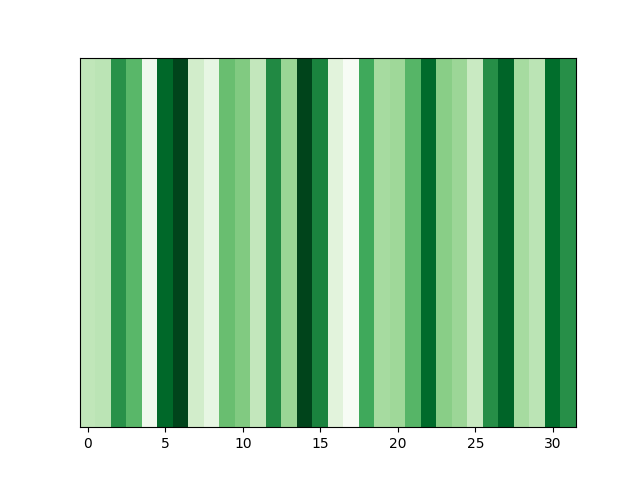
\includegraphics[width=8cm]{happiness.png}
    \caption{Embedding of "Happiness"}
    \label{fig:height}
    \end{center}
\end{figure}

\begin{figure}
    \begin{center}
    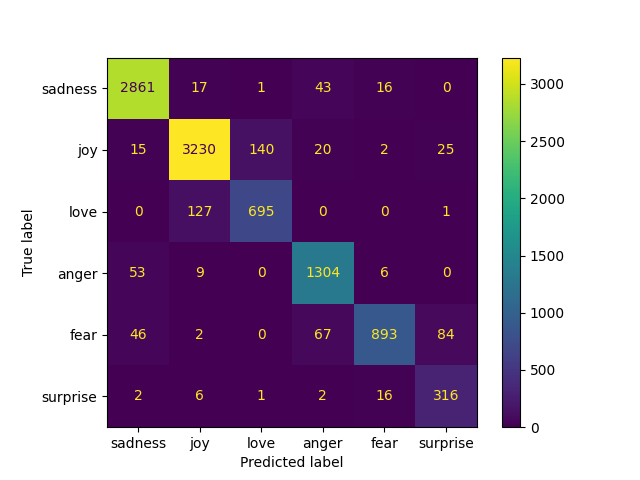
\includegraphics[width=8cm]{cm.png}
    \caption{Confusion Matrix for Model 2}
    \label{fig:height}
    \end{center}
\end{figure}

After fitting our GRU model, we found that it achieved an accuracy of 93\%. Figure 1 displays the learning curves of our model. We observed that even after five epochs, the accuracy and val-accuracy curves are still close together. The loss curves, which measure the error between predicted output and actual answer, show a similar behavior. Overall, there is a lack of evidence that our model is overfitting.

We created a second model using a simple RNN layer to observe how much the GRU model improves on the Simple RNN model. After fitting the Simple RNN model, we found an accuracy of around 88\%, and improvement of around 4\%. Like with the GRU model, we do have any evidence that the Simple RNN model is overfitting.

To observe what our model is actually learning, we compared embedding of various words. Figure 3, 4 and 5 are color representations of the learned weights of the embeddings for the words "sad," "depressed," and "unhappy." Cells that are green represent positive weights, while cells that are white represent negative weights. "Sad," "depressed," and "unhappy" are all adjectives that desribe the same feeling, so it is noteworthy that our model gave them very similar weights. To further analyzed the embedding weights, we compared the embeddings of the same word in different parts of speech as well as the embeddings of different words but both in the same parts of speech.

Comparing Figure 3 ("sad") and Figue 6 ("sadness"), we can see that the pattern between weights 7 and 14 are similar, indicating that these may be the weights that capture sentiment. However, we were not able to find a similar pattern with Figure 7 ("happy") and Figure 8 ("happiness"). However, the embeddings of "happy" and "sad" seem to be similar around weights 18 and 22. The embeddings for "happiness" and "sadness" also show similarity at this range of weights. Thus, it is possible that this range of weights capture parts of speech. Overall, there are evidence that the model is indeed learning the sentiment of each of these words and where they may be placed in a sentence. 

Lastly, we used a confusion matrix of our predicted labels vs. actual labels to evaluate our model for areas of weakness. From Figure 9, we noticed that our model confuses joy and love more often than any other emotions. When the model predicts love, around 17\% of the time it is incorrectly labeling a joyous tweet. Another way of looking at this is that when the tweet is joyous, our model will say that it is loving around 4\% of the time. When the model predicts joy, around 4\% of the time it is incorrectly labeling a joyous tweet. When the tweet is loving, our model will say that it is joyous around 16\% of the time. The emotions "joy" and "love" are very similar, so it follows that our model is likely to mess up when analyzing these types of tweets.

\section{Conclusions}

In this paper, we utilized a Gated Recurrent Unit (GRU)-based deep learning approach for sentiment analysis on a dataset of tweets. While we were able to achieve an impressive 93\% accuracy, there are other areas in which we can explore with this topic. For example, it is possible that sentiment analysis on tweets is a relatively easy problem to solve for GRUs considering tweets are very short (usually less than 100 words). Assessing the robustness of our model would require a dataset of longer prose. Another avenue we could take involve including more kinds of labels on top of the six we used in this paper. Lastly, we could compare the GRU model with other kinds of RNN models, including Long Short Term Memory (LSTM) models and Bi-directional LSTM Model.

\section{Acknowledgements}

To understand and build our GRU model, we used the Geeks for Geeks' "Sentiment Analysis with an Recurrent Neural Networks (RNN)" article. We also used mathplotlib and keras documentations to help us understand how to utilize their libraries. To create our colormaps, we used Copilot to generate instructions (pseudocode) on how to turn a float array into a colormap. To create our confusion matrix, we took the code from Lab 7.

\section{References}
\begin{enumerate}
    \item Elgiriyewithana, Nidula. “Emotions.” \textit{Kaggle}, 5 Feb. 2024, www.kaggle.com/datasets/nelg iriyewithana/emotions. Accessed 06 May 2024.
    \item “Sentiment Analysis with an Recurrent Neural Networks (RNN).” \textit{GeeksforGeeks}, 14 Oct. 2022, www.geeksforgeeks.org/sentiment-analysis-with-an-recurrent-neural-networks-rnn/?ref=lbp. Accessed 06 May 2024. 
\end{enumerate}

\end{document}
